\section{Comparison between DRO and importance weighting}\label{sec:resampling}

Our results above show that strongly-regularized DRO models can be significantly more robust than ERM models.
Here, we show theoretically and empirically that DRO also outperforms a strong importance weighting baseline that is commonly used in machine learning tasks where the train and test distributions differ \citep{shimodaira2000improving, byrd2019effect}.
Recall that in our setting, the test distribution can be any mixture of the group distributions.
For some assignment of weights $w \in \Delta_m$ to groups, an importance-weighted estimator would learn
\begin{align}
  \htw \eqdef \argmin_{\theta \in \Theta} \ \E_{(x,y,g) \sim \hP}[w_g \ \ell(\theta; (x, y))].
\end{align}


\textbf{Empirical comparison.}
We consider an importance-weighted baseline with weights set to the inverse training frequency of each group,
 $w_g = 1 / \E_{g^\prime \sim \hP} [\1(g^\prime = g)]$.
This optimizes for a test distribution with uniform group frequencies
and is analogous to the common upweighting technique for label shifts
\citep{cui2019class, cao2019learning};
intuitively, this attempts to equalize average and worst-group error by upweighting the minority groups.
Concretely,
we train our weighted model by sampling from each group with equal probability \citep{shen2016relay},
since a recent study found this to be more effective than similar reweighting/resampling methods \citep{buda2018systematic}.

Unlike group DRO, upweighting the minority groups does not necessarily yield uniformly low training losses across groups in practice, as some groups might be easier to fit than others.
To compare upweighting (UW) with ERM and DRO,
we train models across the same grid of $\Ltwo$ penalty strengths and early stopping at the epoch with best worst-group validation accuracy (\reftab{benchmark}).%
\footnote{To avoid advantaging the DRO models by allowing them to tune additional hyperparameters,
we restrict our search for group adjustments to the one $\Ltwo$ penalty strength used in \refsec{experiments_adjustments}. See \refapp{model_details}.}
In CelebA and Waterbirds,
upweighting performs much better than ERM but is slightly outperformed by DRO.
However, upweighting fails on MultiNLI, achieving lower average and worst-group accuracies than even ERM.
With upweighting, it appears that the rare group is overemphasized and extremely low training accuracy is achieved for that group at the cost of others.


\begin{table}[th]
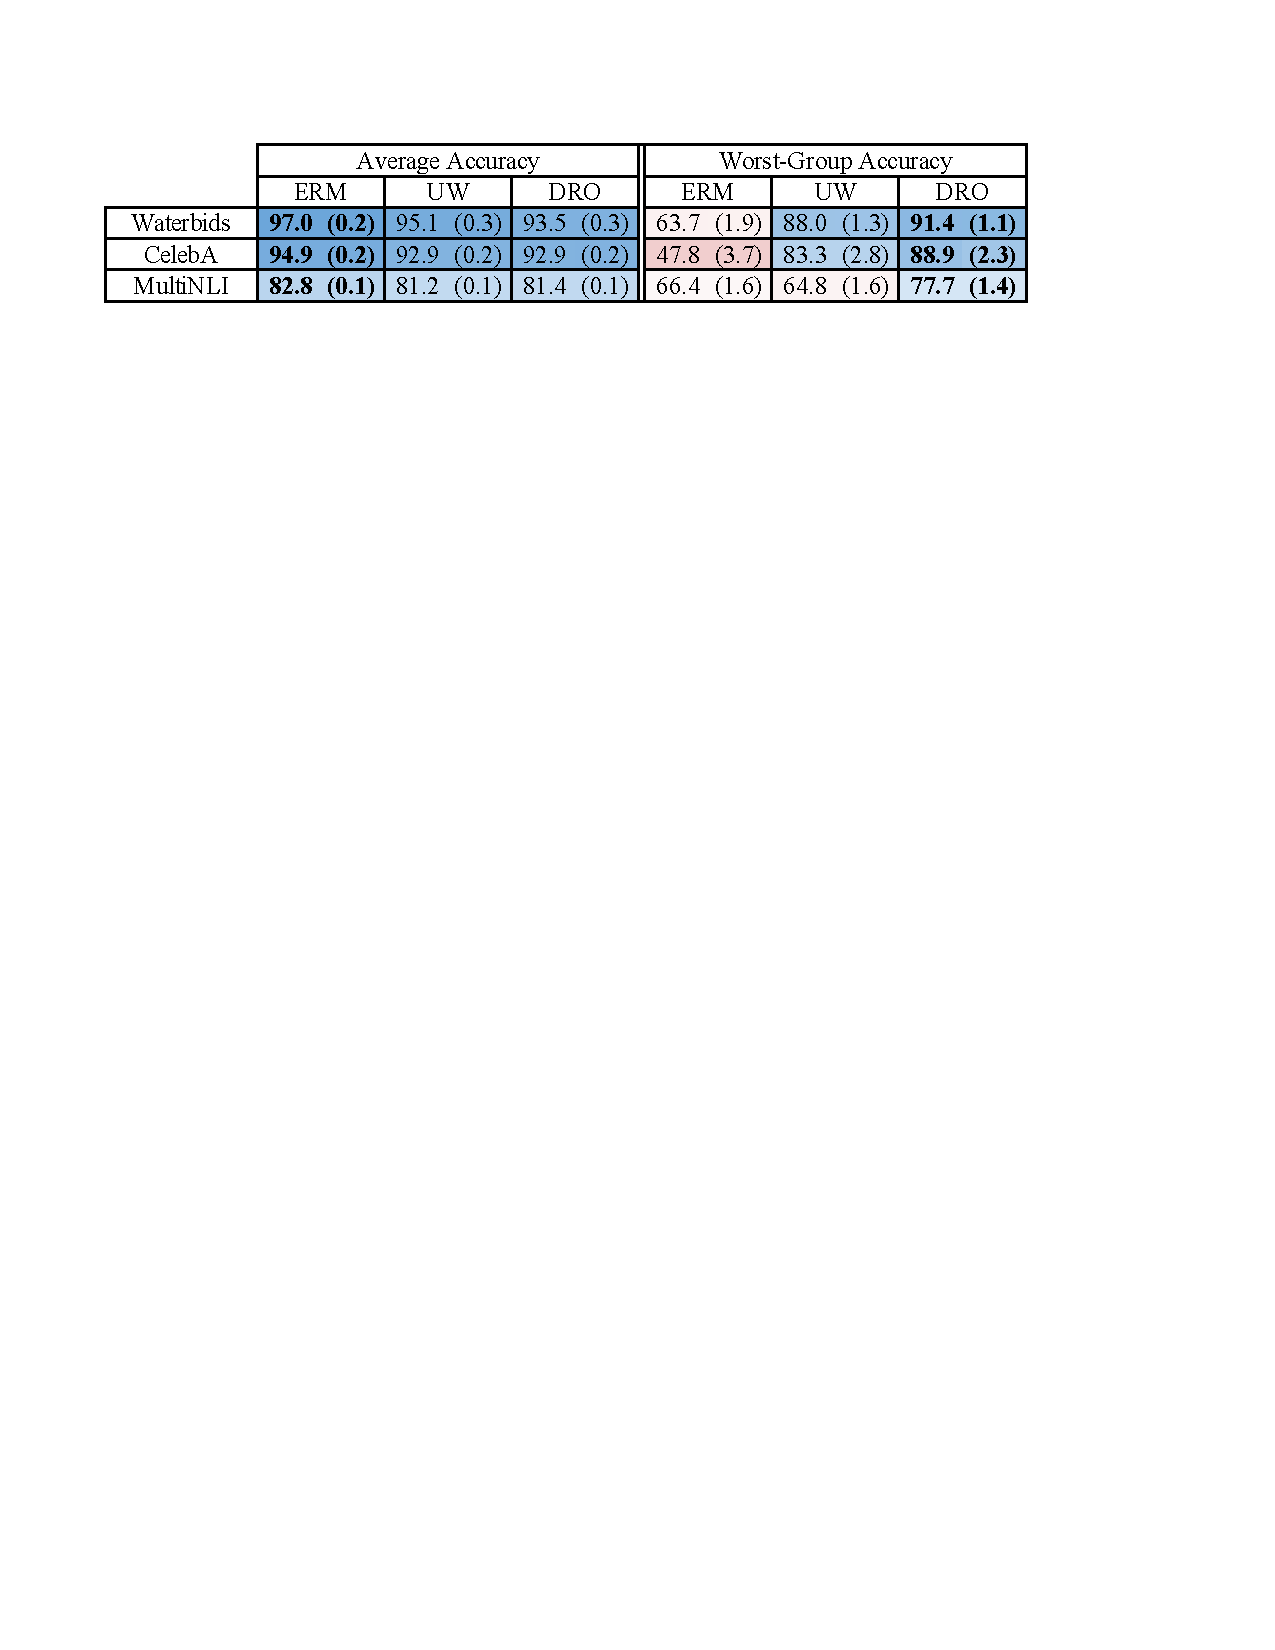
\includegraphics[width=0.8\textwidth]{figs/table_3.pdf}
\caption{Comparison of ERM, upweighting (UW), and group DRO models, with binomial standard deviation in parenthesis. For each objective, we grid search over $\Ltwo$ penalty strength, number of epochs, and group adjustments and report on the model with highest validation accuracy.
These numbers differ from the previous tables because of the larger grid search.
  }
\label{tab:benchmark}
\end{table}

\begin{figure}[th]
  \centering
  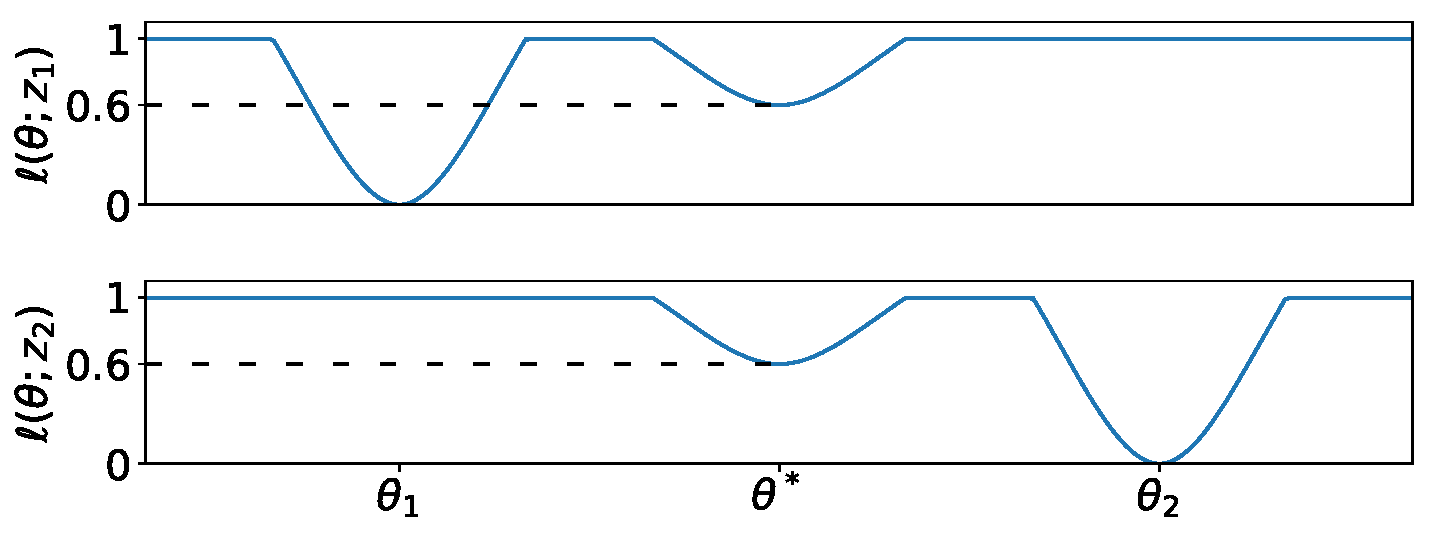
\includegraphics[width=0.6\textwidth]{figs/counterexample.pdf}
  \caption{
    Toy example illustrating that DRO and importance weighting are not equivalent. The DRO solution is $\theta^*$, while any importance weighting would result in solutions at $\theta_1$ or $\theta_2$.
  }\label{fig:DRO_counterexample}
\end{figure}


\textbf{Theoretical comparison.}
Should we expect
importance weighting
to learn models with good worst-case loss?
We show that importance weighting and DRO can learn equivalent models in the convex setting under some importance weights, but not necessarily when the models are non-convex.

We analyze the general framework of having weights $w(z)$ for each data point $z$, which is more powerful than the specific choice above of assigning weights by groups.
By minimizing the weighted loss
$\E_{z \sim P}[w(z) \ell(\theta; z)]$ over some source distribution $P$,
we can equivalently minimize the expected loss
$\E_{z \sim Q}[\ell(\theta; z)]$ over a target distribution $Q$
where $Q(z) \propto w(z)P(z)$.
However, we want good worst-case performance over a family of $Q \in \sQ$,
instead of a single $Q$.
Are there weights $w$ such that the resulting model $\htw$ achieves optimal worst-group risk?
In the convex regime, standard duality arguments show that this is the case (see \refapp{proof_convex} for the proof):

\begin{proposition}\label{prop:convex-reweight}
  Suppose that the loss $\ell(\cdot; z)$ is continuous and convex for all $z$ in $\sZ$,
  and let the uncertainty set $\sQ$ be a set of distributions supported on $\sZ$.
  Assume that $\sQ$ and the model family $\Theta \subseteq \R^d$ are convex and compact,
  and let $\theta^* \in \Theta$ be a minimizer of the worst-group objective $\sR(\theta)$.
  Then there exists a distribution $Q^* \in \sQ$ such that $\theta^* \in \argmin_\theta \E_{z \sim Q^*} [\ell(\theta;z)]$.
\end{proposition}

However, this equivalence breaks down when the loss $\ell$ is non-convex:

\begin{counterexample}
Consider a uniform data distribution $P$ supported on two points $\sZ = \{z_1, z_2\}$,
and let $\ell(\theta; z)$ be as in \reffig{DRO_counterexample},
with $\Theta = [0, 1]$.
The DRO solution $\theta^*$ achieves a worst-case loss of $\sR(\theta^*)=0.6$.
Now consider any weights $(w_1, w_2) \in \Delta_2$ and w.l.o.g.\ let $w_1 \geq w_2$.
The minimizer of the weighted loss
$w_1 \ell(\theta; z_1) + w_2 \ell(\theta; z_2)$
is $\theta_1$, which only attains a worst-case loss of $\sR(\theta^*)=1.0$.
\end{counterexample}

\begin{remark}
  Under regularity conditions, there exists a distribution $Q$ such that $\theta^*$ is a first-order stationary point of $\E_{z \sim Q} [\ell(\theta;z)]$ (see e.g., \citet{arjovsky2019invariant}).
  However, as the counterexample demonstrates, in the non-convex setting this does not imply that $\theta^*$ actually minimizes $\E_{z \sim Q} [\ell(\theta;z)]$.
\end{remark}

This negative result implies that in the non-convex setting,
there may not be \emph{any} choice of weights $w$
such that the resulting minimizer $\htw$ is robust.
Even if such weights did exist, they depend on $\theta^*$ and obtaining these weights requires that we solve a dual DRO problem, making reweighting no easier to implement than DRO.
Common choices of weights, such as inverse group size, are heuristics that may not yield robust solutions (as observed for MultiNLI in \reftab{benchmark}).
